% Part: sets-functions-relations
% Chapter: arithmetization
% Section:reals

\documentclass[../../../include/open-logic-section]{subfiles}

\begin{document}

\olfileid[fr]{sfr}{arith}{real}
\olsection{La droite réelle}

L'étape suivante consiste à construire les nombres réels à partir des
rationnels. Auparavant, il nous faut comprendre ce qui \emph{distingue}
les réels des rationnels.

Les réels possèdent de nombreuses propriétés communes avec les rationnels.
(Techniquement, ces deux ensembles sont des \emph{corps ordonnés} ; voir
la \olref[check]{orderedfield}.) Si vous avez résolu les
exercices du \olref[sfr][siz][]{chap}, vous savez qu'il y a strictement plus
de réels que de rationnels, c'est-à-dire que $\cardless{\Rat}{\Real}$.
Cantor fut le premier à le démontrer. Mais l'existence de nombres
irrationnels, c'est-à-dire de réels qui ne sont pas rationnels, est connue
depuis environ deux millénaires et demi. En effet :
%\footnote{Le commentaire source affirme que « $\sqrt{2}$ » désigne aussi bien la racine positive que la racine négative, puis annonce qu'il ne considérera que la racine positive dans les pages suivantes. Cette affirmation sur la notation est corrigée dans la note éditoriale ci-dessous.}
\begin{thm}\ollabel{root2irrational}
$\sqrt{2}$ est irrationnel, c'est-à-dire que $\sqrt{2} \notin \Rat$.
\footnote{Précision éditoriale : $\sqrt{2}$ désigne la racine carrée positive de $2$ ; les deux racines de l'équation $x^2=2$ sont $\sqrt{2}$ et $-\sqrt{2}$. Cette précision corrige une note laissée en commentaire dans la source, qui attribuait les deux sens au même symbole.}\end{thm}

\begin{proof}
Supposons, pour raisonner par l'absurde, que $\sqrt{2}$ soit rationnel.
Alors $\sqrt{2} = \nicefrac{m}{n}$ pour des naturels $m$ et $n$
strictement positifs. Choisissons-les de sorte que la fraction soit
irréductible. En réarrangeant, nous obtenons $m^{2} = 2n^{2}$.
Nous pouvons terminer la démonstration de deux manières :

\emph{Premièrement, par un raisonnement géométrique} (dû à Tennenbaum).\footnote{Cette démonstration est rapportée par \cite{Conway2006}.}
Considérons les carrés suivants :
\begin{center}
	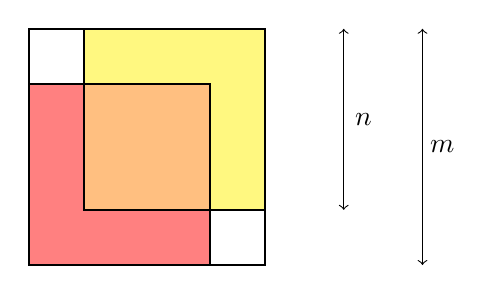
\begin{tikzpicture}
		\draw[thick] (0,0) rectangle (3,3);
		\draw[thick, fill=red!50] (0,0) rectangle (2.3,2.3);
		\draw[thick, fill=yellow!50] (0.7,0.7) rectangle (3, 3);
		\draw[thick, fill=orange!50] (0.7,0.7) rectangle (2.3, 2.3);
		\draw[<->] (4, 0.7)--(4, 3);
		\node at (4.25, 1.85) (n) {$n$};
		\draw[<->] (5, 0)--(5, 3);
		\node at (5.25, 1.5) (m) {$m$};
	\end{tikzpicture}
\end{center}
Puisque $m^2 = 2n^2$, la région où les deux carrés de côté $n$ se
recouvrent a la même aire que la région qu'aucun des deux ne couvre :
l'aire du carré orange est donc égale à la somme des aires des deux
carrés non colorés. Si le carré orange a pour côté $p$ et chacun des
carrés non colorés pour côté $q$, alors $p^2 = 2q^2$. Ainsi,
$\sqrt{2} = \nicefrac{p}{q}$, avec $p < m$, $q < n$ et $p, q \in
\Nat$.\footnote{Précision éditoriale : $p=2n-m$ et $q=m-n$. L'égalité $m^2=2n^2$, avec $m,n>0$, donne $n<m<2n$ ; ainsi $p,q>0$, $p<m$ et $q<n$. Les longueurs sont donc bien des naturels strictement positifs. Ces expressions des côtés sont explicites dans la présentation de Conway.}
Cela contredit la minimalité de $m$ et de $n$, assurée par le choix
d'une fraction irréductible.

\emph{Deuxièmement, par un raisonnement algébrique.} Comme
$m^{2} = 2n^{2}$, $m$ est pair. (On montre aisément que, si $x$ est
impair, alors $x^2$ est impair.) Il existe donc $r \in \Nat$ tel que
$m = 2r$. En réarrangeant, nous obtenons $2r^2 = n^2$,
		%\begin{align*}
		%	(2q)^{2} &= 2n^{2}\\
		%	4q^{2} &= 2n^{2}\\
		%	2q^{2} &= n^{2}
		%\end{align*}
et $n$ est donc lui aussi pair. Les deux nombres $m$ et $n$ étant
pairs, la fraction $\nicefrac{m}{n}$ \emph{peut} encore être simplifiée.
C'est une contradiction !{}
\end{proof}

Cette preuve par le dessin nous permet au passage de revenir à la
\olref[his][set][mythology]{sec}. Tennenbaum (1927--2006) était un
mathématicien tout à fait moderne ; pourtant, sa démonstration est
incontestablement élégante, parfaitement rigoureuse et fondée sur
l'intuition géométrique !{}

Quoi qu'il en soit, les réels forment un ensemble «~plus riche~» que les
rationnels. En un certain sens, les rationnels présentent des «~lacunes~»
que les réels comblent. Weierstrass a reconnu que cette idée s'exprime
par une propriété qui distingue les réels des rationnels : la
\emph{propriété de la borne supérieure}. Elle affirme que
\emph{tout ensemble non vide de nombres réels qui admet un majorant
admet un plus petit majorant.}

Il est facile de voir que les rationnels ne possèdent pas cette
propriété. Considérons par exemple l'ensemble des rationnels
strictement inférieurs à $\sqrt{2}$, c'est-à-dire :
\[
	\Setabs{p \in \Rat}{p^2 < 2 \text{ ou }p < 0}
\]
Cet ensemble admet un majorant rationnel : tous ses !!{element}s sont,
par exemple, strictement inférieurs à $3$. Mais quel serait son plus
petit majorant ? Nous voudrions répondre «~$\sqrt{2}$~» ; or nous venons
de voir que $\sqrt{2}$ n'est \emph{pas} rationnel. Et il n'existe pas
de \emph{plus petit} rationnel strictement supérieur à $\sqrt{2}$.
Cet ensemble admet donc un majorant rationnel, mais pas de plus petit
majorant rationnel. Les rationnels ne possèdent ainsi pas la propriété
de la borne supérieure.\footnote{Correction typographique : un signe $<$ parasite suivait le marqueur désignant les éléments dans la source. Il est retiré ; la comparaison avec $3$ reste inchangée.}

En revanche, la propriété de la borne supérieure répond à ce que nous
attendons intuitivement du continu. Nous ne voulons pas seulement que
$\sqrt{2}$ soit un nombre réel : nous voulons combler toutes les
«~lacunes~» de la droite rationnelle, et que le continu lui-même n'en
présente aucune. C'est précisément ce qu'assure cette propriété.

\end{document}
